% Forrás: Fleiner Tamás gyakorlat

\documentclass[tikz]{standalone}
\usepackage{tikz}
\usetikzlibrary{positioning, graphs}
\usetikzlibrary{graphs.standard}
\begin{document}
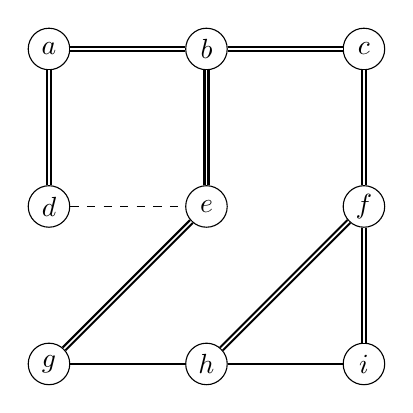
\begin{tikzpicture}
		[vertex/.style={draw,circle,inner sep = 0mm, minimum size = 15},
         edgelabel/.style = {fill = white, inner sep = 2, font=\small}]

        \node[vertex] (a) at (0, 0) {$a$};
        \node[vertex] (b) at (2, 0) {$b$};
        \node[vertex] (c) at (4, 0) {$c$};
        \node[vertex] (d) at (0, -2) {$d$};
        \node[vertex] (e) at (2, -2) {$e$};
        \node[vertex] (f) at (4, -2) {$f$};
        \node[vertex] (g) at (0, -4) {$g$};
        \node[vertex] (h) at (2, -4) {$h$};
        \node[vertex] (i) at (4, -4) {$i$};
-
        \draw[-, thick, double] (a) to (b);
        \draw[-, thick, double] (b) to (c);
        \draw[-, thick, double] (a) to (d);
        \draw[-, thick, double] (b) to (e);
        \draw[-, thick, double] (c) to (f);
        \draw[-, thick, double] (e) to (g);
        \draw[-, thick, double] (f) to (h);
        \draw[-, thick, double] (f) to (i);
        
        \draw[-, dashed] (d) to (e);
        \draw[-] (g) to (h);
        \draw[-] (h) to (i);
		
\end{tikzpicture}
\end{document}